
\documentclass[10pt, conference]{IEEEtran}

\usepackage{listings}

% *** CITATION PACKAGES ***
%
%\usepackage{cite}
% cite.sty was written by Donald Arseneau
% V1.6 and later of IEEEtran pre-defines the format of the cite.sty package
% \cite{} output to follow that of IEEE. Loading the cite package will
% result in citation numbers being automatically sorted and properly
% "compressed/ranged". e.g., [1], [9], [2], [7], [5], [6] without using
% cite.sty will become [1], [2], [5]--[7], [9] using cite.sty. cite.sty's
% \cite will automatically add leading space, if needed. Use cite.sty's
% noadjust option (cite.sty V3.8 and later) if you want to turn this off.
% cite.sty is already installed on most LaTeX systems. Be sure and use
% version 4.0 (2003-05-27) and later if using hyperref.sty. cite.sty does
% not currently provide for hyperlinked citations.
% The latest version can be obtained at:
% http://www.ctan.org/tex-archive/macros/latex/contrib/cite/
% The documentation is contained in the cite.sty file itself.

% *** GRAPHICS RELATED PACKAGES ***
%
\usepackage{subimages}
\setfigdir{figs}


% *** MATH PACKAGES ***
%
\usepackage[cmex10]{amsmath}
% A popular package from the American Mathematical Society that provides
% many useful and powerful commands for dealing with mathematics. If using
% it, be sure to load this package with the cmex10 option to ensure that
% only type 1 fonts will utilized at all point sizes. Without this option,
% it is possible that some math symbols, particularly those within
% footnotes, will be rendered in bitmap form which will result in a
% document that can not be IEEE Xplore compliant!
%
% Also, note that the amsmath package sets \interdisplaylinepenalty to 10000
% thus preventing page breaks from occurring within multiline equations. Use:
\interdisplaylinepenalty=2500
% after loading amsmath to restore such page breaks as IEEEtran.cls normally
% does. amsmath.sty is already installed on most LaTeX systems. The latest
% version and documentation can be obtained at:
% http://www.ctan.org/tex-archive/macros/latex/required/amslatex/math/
\usepackage{amsthm}
\newtheorem{definition}{Definition}

% *** SPECIALIZED LIST PACKAGES ***
%
%\usepackage{algorithmic}
% algorithmic.sty was written by Peter Williams and Rogerio Brito.
% This package provides an algorithmic environment fo describing algorithms.
% You can use the algorithmic environment in-text or within a figure
% environment to provide for a floating algorithm. Do NOT use the algorithm
% floating environment provided by algorithm.sty (by the same authors) or
% algorithm2e.sty (by Christophe Fiorio) as IEEE does not use dedicated
% algorithm float types and packages that provide these will not provide
% correct IEEE style captions. The latest version and documentation of
% algorithmic.sty can be obtained at:
% http://www.ctan.org/tex-archive/macros/latex/contrib/algorithms/
% There is also a support site at:
% http://algorithms.berlios.de/index.html
% Also of interest may be the (relatively newer and more customizable)
% algorithmicx.sty package by Szasz Janos:
% http://www.ctan.org/tex-archive/macros/latex/contrib/algorithmicx/


% *** ALIGNMENT PACKAGES ***
%
%\usepackage{array}
% Frank Mittelbach's and David Carlisle's array.sty patches and improves
% the standard LaTeX2e array and tabular environments to provide better
% appearance and additional user controls. As the default LaTeX2e table
% generation code is lacking to the point of almost being broken with
% respect to the quality of the end results, all users are strongly
% advised to use an enhanced (at the very least that provided by array.sty)
% set of table tools. array.sty is already installed on most systems. The
% latest version and documentation can be obtained at:
% http://www.ctan.org/tex-archive/macros/latex/required/tools/


%\usepackage{mdwmath}
%\usepackage{mdwtab}
% Also highly recommended is Mark Wooding's extremely powerful MDW tools,
% especially mdwmath.sty and mdwtab.sty which are used to format equations
% and tables, respectively. The MDWtools set is already installed on most
% LaTeX systems. The lastest version and documentation is available at:
% http://www.ctan.org/tex-archive/macros/latex/contrib/mdwtools/


% IEEEtran contains the IEEEeqnarray family of commands that can be used to
% generate multiline equations as well as matrices, tables, etc., of high
% quality.


%\usepackage{eqparbox}
% Also of notable interest is Scott Pakin's eqparbox package for creating
% (automatically sized) equal width boxes - aka "natural width parboxes".
% Available at:
% http://www.ctan.org/tex-archive/macros/latex/contrib/eqparbox/



% *** PDF, URL AND HYPERLINK PACKAGES ***
%
\usepackage{hyperref}
% *** Do not adjust lengths that control margins, column widths, etc. ***
% *** Do not use packages that alter fonts (such as pslatex).         ***
% There should be no need to do such things with IEEEtran.cls V1.6 and later.
% (Unless specifically asked to do so by the journal or conference you plan
% to submit to, of course. )


% correct bad hyphenation here
\hyphenation{op-tical net-works semi-conduc-tor}


\begin{document}
%
% paper title
% can use linebreaks \\ within to get better formatting as desired
\title{Specular Fading over Distance on Wrinkled Surfaces}

%-------------------------------------------------------------------------
% change the % on next lines to produce the final camera-ready version
\newif\iffinal
\finalfalse
%\finaltrue
\newcommand{\jemsid}{114562}
%-------------------------------------------------------------------------

% author names and affiliations
% use a multiple column layout for up to two different
% affiliations

\iffinal
  \author{%
    \IEEEauthorblockN{Troy Kohwalter, Esteban Clua, Leandro Fernandes}
    \IEEEauthorblockA{%
      Instituto de Computação\\
      Universidade Federal Fluminense\\
      Niterói – RJ, Brazil\\
      {tkohwalter, esteban, laffernandes}@ic.uff.br}
  }
\else
  \author{Sibgrapi paper ID: \jemsid \\ }
\fi


%-------------------------------------------------------------------------
% Special Sibgrapi teaser
\teaser{%
	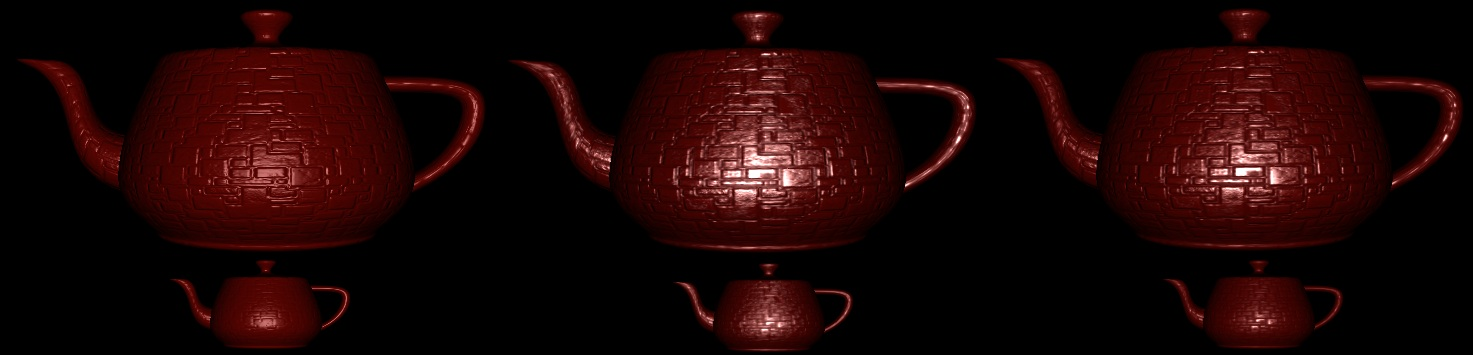
\includegraphics[width=0.99\textwidth]{figs/Teaser.png}
	\caption{Bump mapping with traditional Blinn-Phong shading (left), LEAN mapping (center), and our model (right) applied on teapots at different distances from the observer (top and bottom). In contrast to other approaches, our technique is capable to reproduce the natural fading of the specular component over distance without loss of contrast (left) or without the introduction of additional energy (center).}
	\label{fig:Teaser}
}
%-------------------------------------------------------------------------


% make the title area
\maketitle


\begin{abstract}
Blinn-Phong shading model provides rich visual experience for bumped surfaces when used with traditional normal mapping techniques. However, when the observer is far from the surface, the bumped regions may become blurred and disappear, thus making the surface duller than it is. The Linear Efficient Antialiased Normal (LEAN) mapping is a well stablished tentative to correct this issue. However, in that approach the specular highlight intensity of small bumps is unaffected by distance, leading to brighter specular highlights than one would expect. We present an extension of LEAN mapping where the excess of energy in the specular highlight is corrected by introducing a fading term during the computation of the specular component of the illumination model. This term produces more convincing specular effects for real time graphics applications such as games and virtual reality.

% DO NOT USE SPECIAL CHARACTERS, SYMBOLS, OR MATH IN YOUR TITLE OR ABSTRACT.
%
\end{abstract}

\begin{IEEEkeywords}
bump mapping; normal mapping; LEAN mapping; specular ilumination;

\end{IEEEkeywords}


\IEEEpeerreviewmaketitle


% Wherever Times is specified, Times Roman or Times New Roman may be used. If neither is available on your system, please use the font closest in appearance to Times. Avoid using bit-mapped fonts if possible. True-Type 1 or Open Type fonts are preferred. Please embed symbol fonts, as well, for math, etc.

%==========================================
%==========================================


%==========================================
\section{Introduction}
%
To create the illusion of details in surfaces, artists usually create and apply normal maps at the mesh description. In many cases, these maps contain random bumps to better simulate rough surface materials at close range. The surface of these perceived roughnesses should be the same when displayed at different distances to the viewer. However, due to filtering issues regarding non-regular and near-stochastic patterns combined to inappropriate shading models, the shading wrinled surfaces are often inconsistent across different levels of detail and distance. This happens because the shading model at the coarsest level of detail does not correspond to the mapped bumps at a finer level of detail. Traditional filterings and mip-mapping techniques may produce inconsistent results, with false atenuation of the specular effect.

Bump mapping was originally introduced by Blinn~\cite{Blinn:1978:SWS:800248.507101}. He demonstrated how to simulate wrinkled surfaces by only perturbing the normal vector without changing the underlying surface itself. The perturbed normal replaces the original normal vector of the surface while lighting is computed. For about thirty years, the bump mapping has been an effective method for adding apparent detail to a surface. Programmable GPUs made this technique available for real time rendering, being a common feature in almost any 3D game.

Unfortunately, bump mapping has serious drawbacks with filtering and antialiasing. When the bumps are viewed at a distance, the standard mipmapping technique for bump map can work well for diffuse shading~\cite{Kilgard00apractical}. However, it fails to capture changes in specularity. When looking far away, the result will be a shiny and bump-less surface, appearing as if it were duller. Many techniques that tries to solve the highlight aliasing problem were proposed, but most of them require pre-processing stages~\cite{Cabral:1987:BRF:37401.37434, Becker:1993:STB:166117.166141, Westin:1992:PRF:133994.134075}. To correct this issue, a new mapping approach called Linear Efficient Antialiased Normal (LEAN) mapping was developed by Olano and Baker~\cite{Olano:2010:LM:1730804.1730834}. With this approach, the bumps are preserved at high distances. Nevertheless, the specular highlights produced by small bumps are also visible, making the surface artificially shiny.


%-------------------------------------------------------------------------
\paragraph*{Contributions}
%
This paper describes an improvement of the LEAN mapping. By introducing a fading component in the computations we show that it is possible to reduce the specular highlight according to the distance of the object. For this purpose, we use the original LEAN mapping in order to avoid the blurring of the bump surface and propose a modification to make the necessary change in the specular highlight, preventing the inclusion of additional energy on the shiny effect.

The remaining of the paper is organized as follows: Section~\ref{sec:related_work} presents some ground basement of previews works in the area, as well as an overview of the proposed method. Section~\ref{sec:specular_fading} presents our modified method. Section~\ref{sec:implementation} and Section~\ref{sec:results} discusses implementation details and obtained results. Section~\ref{sec:conclusion} concludes the paper with some observations and directions for future exploration.
%==========================================
\section{Related Work}
\label{sec:related_work}
%
There are many approaches that model how light reflects at an opaque surface. One of the first well established models was proposed by Blinn~\cite{Blinn:1977:MLR:563858.563893}, which used a simple shading equation based on microfacets to represent micro details as a bidirectional reflectance distribution function (BRDF). Cook and Torrance~\cite{Cook:1982:RMC:357290.357293} have presented a microfacet-based BRDF model which also added shadowing and a Fresnel term to make the representation of metallic and plastic materials more realistic. In contrast to previous work, Ward~\cite{Ward:1992:MMA:133994.134078} has developed a BRDF modeling anisotropic Gaussian distribution of microfacet, and Ashikhmin et al.~\cite{Ashikmin:2000:MBG:344779.344814}  have developed a way of generating reflection models with arbitrary normal distributions.

While micro details of opaque materials can be represented by BRDFs, small bumps on the underlying surface need a more descriptive representation. Blinn~\cite{Blinn:1978:SWS:800248.507101} was the first to to use a height field mapped to the surface to model small (not micro) details on objects represented by coarse triangular meshes. From the height information mapped to a given point on the surface and the normal vector on that point (computed from the original mesh), he demonstrated how to perturb and replace the original normal in order to simulate wrinkles on the surface. Cohen et al.~\cite{Cohen:1998:AS:280814.280832} extended Blinn's ideas and has used textures to store normal vectors and map them directly to the surfaces, avoiding the computation of perturbed normal from a height map. This technique is called Normal Mapping.

Normal Mapping has been combined with BRDFs in games and other real-time graphics applications. However, the filtering process implemented by graphics hardware makes the normal vectors fetched from normal maps not suitable for rendering shiny surfaces at different distances from the observer with existing BRDF models. When viewed from distance, the sampled surface normals will be filtered and the result of changing the normal to an average value makes the bumps no longer visible, which causes the impression of a duller surface. This problem was addressed and partially solved by the LEAN mapping~\cite{Olano:2010:LM:1730804.1730834} technique, in which this work was based on.


%-------------------------------------------------------------------------
\subsection{LEAN Mapping}
%
The LEAN mapping~\cite{Olano:2010:LM:1730804.1730834} is a simple model that is compatible with existing filtering for diffuse bumps. It has a low pre-computation and run-time cost while also being compatible with existing BRDFs such as the Blinn-Phong model proposed by Blinn~\cite{Blinn:1977:MLR:563858.563893}.

The LEAN mapping is a modification of Ward's shading model~\cite{Ward:1992:MMA:133994.134078}. In contrast to conventional filtering, the technique requires one additional MIP~\cite{Williams:1983:PP:800059.801126} texture lookup per shading evaluation and also manages to capture antialiasing of the highlight shape and the transition of anisotropic bumps into an anisotropic highlight. In render time, the technique uses an existing height or normal map to generate two auxiliary LEAN map textures on GPU~\cite{Olano:2010:LM:1730804.1730834}.

The use of LEAN mapping with existing Blinn-Phong-based shaders requires the equivalence of the Blinn-Phong model with the symmetric Ward model using a Beckmann distribution. Given a normal vector,~(\ref{eq:n}), retrieved from the normal map and represented in tangent space:
\begin{equation}
	\label{eq:n}
	N = (\vec{b}_{x}, \vec{b}_{y}, \vec{b}_{z})
\end{equation}
the LEAN map textures are computed as:
\begin{align}
	\label{eq:b}
	B &= (\tilde{b}_{x}, \tilde{b}_{y}) = \left(\frac{\vec{b}_{x}}{\vec{b}_{z}}, \frac{\vec{b}_{y}}{\vec{b}_{z}}\right) \text{, and}\\
	\label{eq:m}
	M &= ({\tilde{b}_{x}}^{2}, {\tilde{b}_{y}}^{2}, \tilde{b}_{x}\tilde{b}_{y})
\end{align}
where $\vec{b}$ is the Bump's Normal. The textures sampling the five values described in~(\ref{eq:b}) and~(\ref{eq:m}) gives an anti-aliased, filtered blend of the bumps and specular shading for any view. Refer to~\cite{Olano:2010:LM:1730804.1730834} for details. To store five values in textures, it is required the usage of two texture units, which enables the possibility to store eight values. The remaining three values can be used to store the conventional normal map in order to save computation and improve the quality of the diffuse filtering, instead of reconstructing it. Figs. \ref{fig:Lean1} and \ref{fig:Lean2} illustrates the RGBA from both generated LEAN textures. As observed in~\cite{Kilgard00apractical}, storing the normal map allows the usage of diffuse filtering with a non-normalized normal resulting from texture filtering.

%==========================================
\begin{figure}[h]
	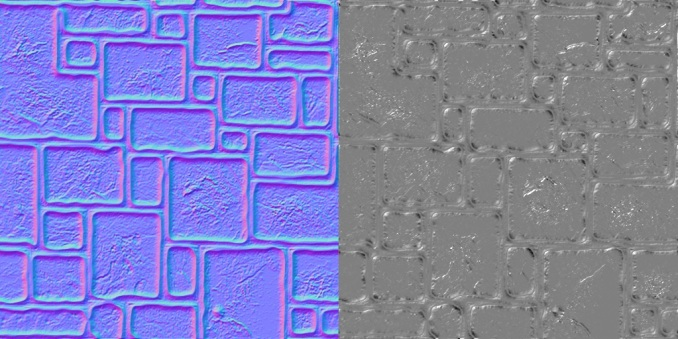
\includegraphics[width=0.49\textwidth]{figs/Lean1.png}
	\caption{First texture generated by LEAN. The first three color channels of the texture (R, G, and B) store the normal map, and the last one (A) stores M.z (defined by~(\ref{eq:m})). Used in Figs.\ref{fig:Teaser}, \ref{fig:sphere}, \ref{fig:ninja}, \ref{fig:torus1} and \ref{fig:LS1}}
	\label{fig:Lean1}
\end{figure}

\begin{figure}[h]
	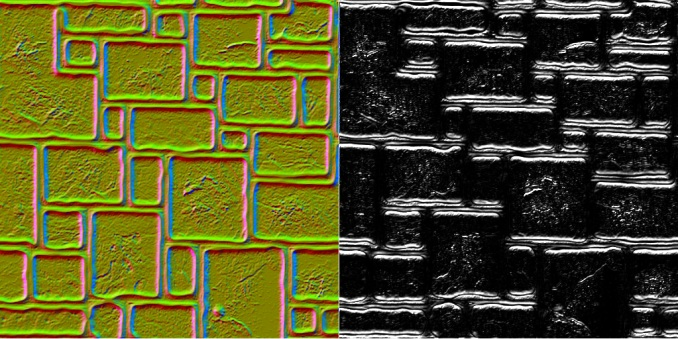
\includegraphics[width=0.49\textwidth]{figs/Lean2.png}
	\caption{Second texture generated by LEAN. The first two color channels (R and G) are used to store B (computed using~(\ref{eq:b})) while the last two channels (BA) store M.x and M.y (computed using~(\ref{eq:m})). Used in Figs.\ref{fig:Teaser}, \ref{fig:sphere}, \ref{fig:ninja}, \ref{fig:torus1} and \ref{fig:LS1}}
	\label{fig:Lean2}
\end{figure}
%==========================================

Given the LEAN textures values, $B$ and $M$ from~(\ref{eq:b}) and~(\ref{eq:m}), respectively, it is possible to compute the covariance $\Sigma$ with~(\ref{eq:covariance}) by using MIP levels and any linear filtering. The covariance controls the size and shape of the highlight center. With the covariance, it is possible to compute $\Sigma^{-1}$ to calculate the LEAN specular term in~(\ref{eq:lean_spec}):

%==========================================
\begin{equation}
	\label{eq:covariance}
	\Sigma = \left( \begin{smallmatrix} M_{x} - B_{x} * B_{x} & M_{z} - B_{x} * B_{y}\\ M_{z} - B_{x} * B_{y} & M_{y} - B_{y} * B_{y} \end{smallmatrix} \right)
\end{equation}

\begin{equation}
	\label{eq:lean_spec}
	\dfrac{1}{2\Pi\sqrt{|\Sigma|}}e^{-0.5(h_{n} - \tilde{b}_{n})^{T} \Sigma^{-1}(h_{n} - \tilde{b}_{n})}
\end{equation}
where $h$ is the half way vector between the vector from the surface toward the viewer and the vector from surface toward the light.

To use LEAN mapping with Blinn-Phong model, it is necessary to add the $1 / s$ term in the final shading when constructing the covariance $∑$, adding it in the $M.x$ and $M.y$ terms~\cite{Olano:2010:LM:1730804.1730834}. Doing so will result in introducing the Blinn-Phong specularity effect in the texture.


%==========================================
\section{Proposed Specular Fading Approach}
\label{sec:specular_fading}
%
The Ward model assumes perfectly reflective microfacets. This feature is inherited by the LEAN mapping technique, leading to specular shininess even on huge distances from the observer. The central contribution of our work is to deal with this problem by introducing a fading term on the computation of the specular component of LEAN mapping approach. Our specular fading term varies according to the camera distance from the object. Both the minimum and maximum highlight specular intensity is configurable. When viewed on close range, the result is identical to LEAN. This new configurable empirical specular fading term is added in a shader as a power of the dot product between Normal and Light vectors.

This new term allows the specular control over distance, which is made during the shading process without significant computational overhead. It acts as an attenuator component based on the distance, reducing the specular highlight. In addition, our distance-based term actually reduces the shiny appearance without interfering with the alpha component or other light model components.

The specular fading control $sf$ is computed as:
%==========================================
\begin{equation}
	\label{eq:sf}
	sf = clamp(1 + (V_{z} * Fade)^{2}, 1, P_max)
\end{equation}
%==========================================
where $V$ is the normalized view vector, $Fade$ is a positive, and greater than zero, parameter used to configure the fading rate, which is also used to adjust to the world scale. The $Fade$ parameter determines the specular energy loss rate by distance ($V_{z}$). $P\_{max}$ is the maximum specular fade desired by the user and is used in conjunction with $clamp$ to control maximum specular loss. This is done so because even if $Fade$ is carefully chosen and controlled in order to avoid illumination glitches, the distance is not. And since specular energy is lost with distance, $clamp$ is used to force $sf$ minimum and maximum values to avoid cases of gaining energy. The $sf$ term must always be greater than one to avoid introducing energy.

The power of two present in~(\ref{eq:sf}) is optional and was used for the sole purpose of increasing the energy loss rate in order to increase visibility in the illutrations presented throughout this paper. Doing so allowed to notice the changes made in the specular highlights while also maintaing the illustrations at a suitable size. This specular fading term, $sf$, is then applied in the intensity of the diffuse light ($NdotL$), as shown by~(\ref{eq:t_spec}), where $Ks$ is the material specular component, $sf$ the specular fading computed by~(\ref{eq:sf}), and $LEAN_{spec}$ is the LEAN specular term calculated from~(\ref{eq:lean_spec}).Because $sf$ is always positive and greater than one, and the intensity of the diffuse light is between zero and one, as $sf$ increases, due to the distance since $Fade$ is constant, the intensity will decrease.
%==========================================
\begin{equation}
	\label{eq:t_spec}
	TotalSpecular = Ks * NdotL^{sf} * LEAN_{spec}
\end{equation}
%==========================================

%==========================================

%-------------------------------------------------------------------------
\section{Implementation}
\label{sec:implementation}

Tests were made in order to compare the new model with the traditional LEAN technique. The tests were performed on a GeForce GTX550Ti, installed in a Windows 7 64-bit machine. The recorded frames per second (fps) were ranging from 1000 to 1600, depending on the distance, for both methods for a square model of 256 triangles and 200 vertices. The difference in performance was barely noticiable between the two techniques. Another geometric model used on the tests was a torus (\figref{torus1}), which is comprised of 2944 triangles and 1884 vertices, however the difference in performance was also barely noticiable. Even with the teapot model containing 79600 triangles and 44366 vertices (\figref{LS1}), the frame rates varied from 570 to 790 fps, depending on the distance, with a difference of approximately 5 fps between techniques.

In our implementation we adapted the equation in the original LEAN shader. Our GLSL shader is presented in listing~\ref{GLSLCode}. For the LEAN stage, we generated lean maps textures (Figs.\ref{fig:Lean1} and \ref{fig:Lean2}, \ref{fig:Lean21} and \ref{fig:Lean22}) as described in~\cite{Olano:2010:LM:1730804.1730834}, and unpacked $N$ (line 5), $B$, $M$ terms from the textures (lines 11 and 12). We then converted $M$ to $∑$ (line 14) and computed the LEAN specular term (lines 15 to 19). Then we compute the intensity of the diffuse light (line 21) and the diffuse component (line 22). After this process, we compute the specular fading $sf$ (lines 24 to 27), the fresnel component (line 29) and the final specular component (line 30). Lastly, the final color using the diffuse and specular components with the light color (line 32).

%==========================================
\lstset{basicstyle=\footnotesize,xleftmargin=20pt,numbers=left, breaklines=true, language=C, caption=GLSL pseudo code for specular fading applied in LEAN shader in tangent space., label=GLSLCode}
\begin{lstlisting}
vec3 fvLightDirection = normalize(LightDirection);
vec3 fvViewDirection = normalize(ViewDirection);
vec3 Half = normalize(fvViewDirection + fvLightDirection);
vec4 t1 = texture2D(Lean1, gl_TexCoord[0].st);
vec3 Normal = vec3(t1.xyz) * 2.0 - 1.0;
// Equivalence for the Blinn-Phong is 1 / s, where s is the specular expoent.
// This is done here to remove the dependancy on the lean map creation.
float equivalence = 1.0 / MaterialShininess;
// Unpack B and M
vec4 t2 = texture2D(Lean2, gl_TexCoord[0].st);
vec2 B = (t2.xy * 2.0 - 1.0);
vec3 M = vec3(t2.zw + equivalence, t1.w * 2.0 - 1.0);
// Convert M to E
vec3 E = M - vec3(B * B, B.x * B.y);
float Det = E.x * E.y - E.z * E.z;
// Compute LEAN Specular term
vec2 h = Half.xy / Half.z - B;
float e = (h.x * h.x * E.y + h.y * h.y * E.x - 2.0 * h.x * h.y * E.z);
float LEAN_spec = (Det <= 0.0) ? 0.0 : exp(-0.5 * e / Det) / sqrt(Det);
// Normal dot LightDirection
float NdotL = clamp (dot (Normal, fvLightDirection , 0.0, 1.0);
fvTotalDiffuse = fvMaterialDiffuse * NdotL;
// Spec Fading Computation
float sf = 1.0 + (pow(ViewDirection.z * Fade, 2.0) );
sf = clamp(sf, 1.0, P_max);
// Add specFading to Specular component
fvTotalSpecular = fvMaterialSpecular * pow(NdotL, sf) * LEAN_spec;
// Compute Fresnel
float fFresnel = clamp(FresnelBias + (FresnelScale * pow(1.0 - dot(Normal, fvViewDirection), 5.0)), 0.0, 1.0);
fvTotalSpecular *= fFresnel;
// Final Color
color = (fvTotalDiffuse + fvTotalSpecular).xyz * LightColor.xyz;
\end{lstlisting}
%==========================================

\section{Result display}
\label{sec:results}
%
While comparing LEAN map with our proposed model, it is possible to notice the difference on specular highlight when the distance between the camera and the object changes. The generated LEAN maps from Figs.\ref{fig:Lean1} and \ref{fig:Lean2}, \ref{fig:Lean21} and \ref{fig:Lean22} were used to generate Figs. \ref{fig:sphere}, \ref{fig:ninja}, \ref{fig:torus1}, \ref{fig:torus2}, \ref{fig:teapot1}, \ref{fig:terrain1} and \ref{fig:terrain2} to illustrate the usage of specular fading, LEAN and bump mapping. Fig.\ref{fig:LS1}, which also used Figs.\ref{fig:Lean1} and \ref{fig:Lean2}, also show the difference between normal LEAN technique and LEAN with specular fading, but starting at a closer range. As shown by these figures when using specular fading, the farther the object is from the camera, the lower the specular highlight is. This happens because of the attenuator component based on the distance.
%==========================================
\begin{figure}[here]
	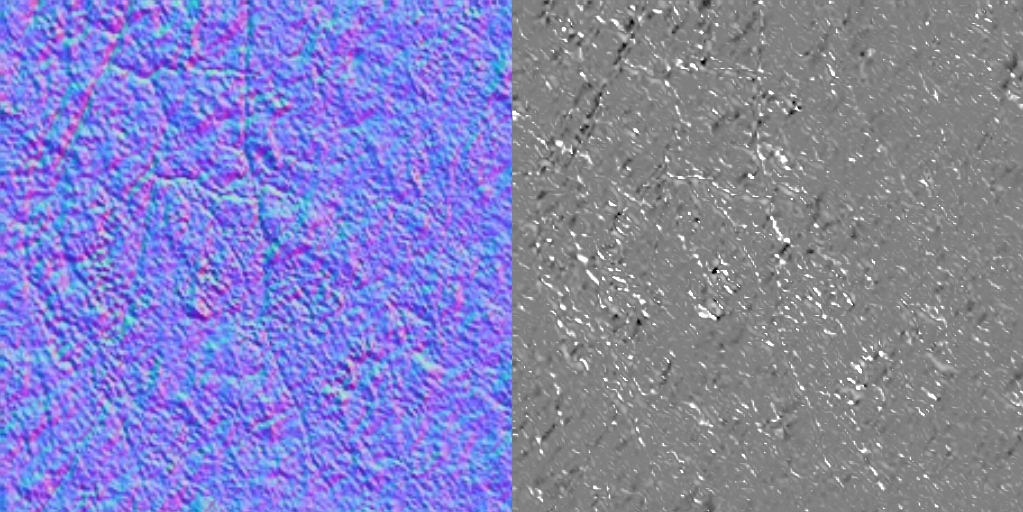
\includegraphics[width=0.49\textwidth]{figs/Lean21.png}
	\caption{First LEAN texture generated for Figs.\ref{fig:torus2}, \ref{fig:teapot1}, \ref{fig:terrain1} and \ref{fig:terrain2}}
	\label{fig:Lean21}
\end{figure}

\begin{figure}[here]
	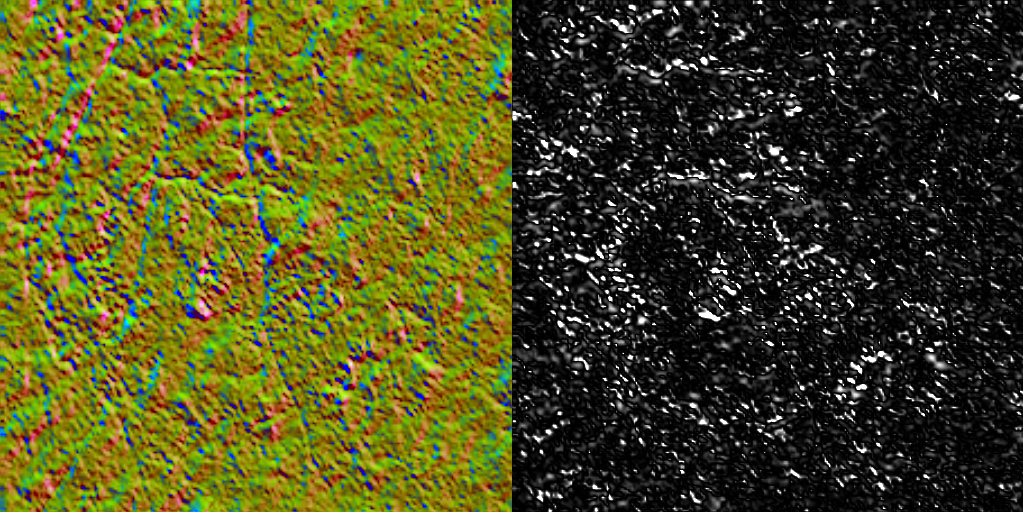
\includegraphics[width=0.49\textwidth]{figs/Lean22.png}
	\caption{Second LEAN texture generated for Figs.\ref{fig:torus2}, \ref{fig:teapot1}, \ref{fig:terrain1} and \ref{fig:terrain2}}
	\label{fig:Lean22}
\end{figure}

\begin{figure}[!h]
	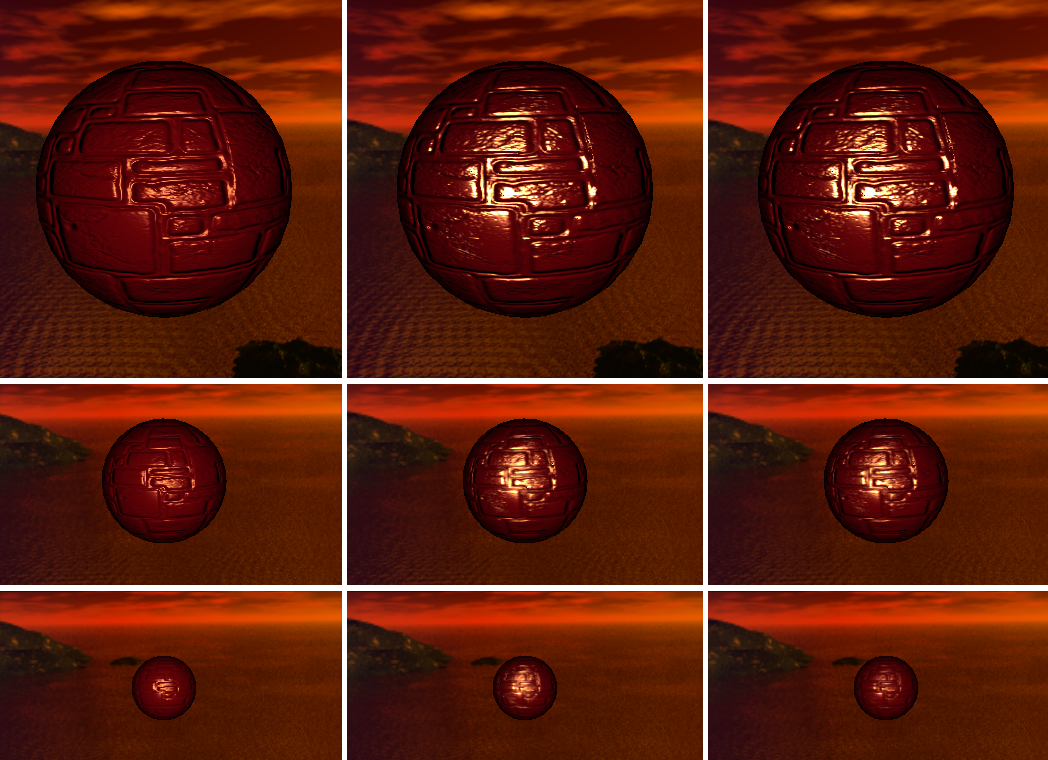
\includegraphics[width=0.49\textwidth]{figs/sphere.png}
	\caption{Comparison between Bump Mapping (left column), LEAN mapping (center), and Specular Fading (right column) using a sphere model. Notice the difference in the specular highlights. At close range, it is very similar to LEAN's, but as the distance increases, the highlight diminishes while keeping the bump aspect of the surface.}
	\label{fig:sphere}
\end{figure}
%==========================================
%fog
This specular fading also corrects the specular highlight from fog algorithms, which only changes the alpha component making it transparent over distance. Notice that this method only attenuate the specular highlight, so it can be used in conjunction with distance fog without problems, allowing the fog algorithm to fade the object while changing the specular.
%==========================================
\begin{figure}[h]
	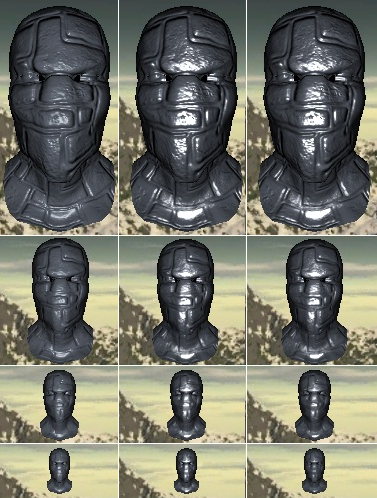
\includegraphics[width=0.49\textwidth]{figs/ninja.png}
	\caption{Another comparsison between approaches but using a ninja head model. Notice the difference of the specular highlights as the distance increases.}
	\label{fig:ninja}
\end{figure}

\begin{figure}[h]
	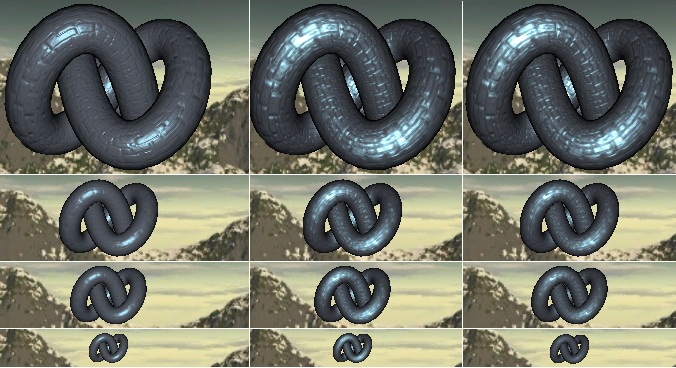
\includegraphics[width=0.49\textwidth]{figs/torus1.png}
	\caption{Another comparsison between approaches, with a torus model and a different specular light color.}
	\label{fig:torus1}
\end{figure}

\begin{figure}[h]
	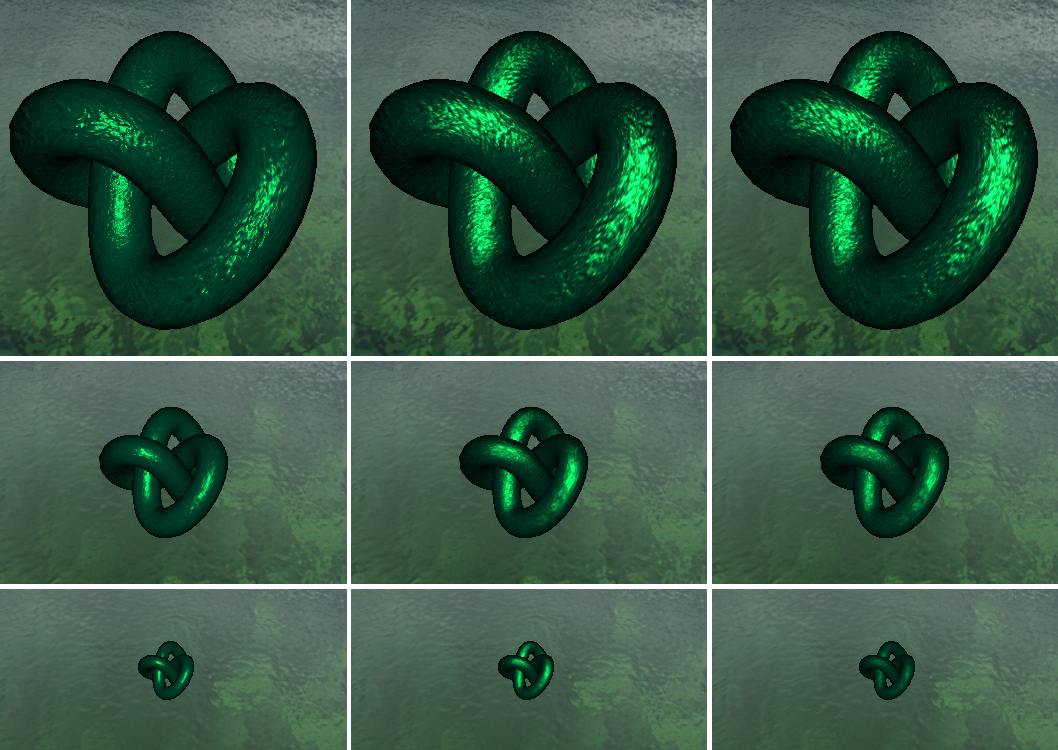
\includegraphics[width=0.49\textwidth]{figs/torus2.png}
	\caption{Another comparison between approaches. Still using the torus model but with different colors and bumps.}
	\label{fig:torus2}
\end{figure}

%==========================================
%==========================================
\section{Conclusion}
\label{sec:conclusion}
%
This paper extended the LEAN mapping technique in order to deal with its problems with excessive specular highlight over distances. The proposed solution consist of a fading term that modules the shininess of the material. Since our fading only affects the specular term, it can also be used in conjunction with fog algorithms, making so that with the increase of distance, the object will suffer light scattering and gradually lose the specular highlight, increasing the visual appeal.

A performance comparison was made between conventional LEAN mapping and the proposed approach. It was concluded that the computational cost of our technique does not have noticeable impact on frame rate. Therefore, our approach can be used in real time applications such as games and virtual reality.


%==========================================
\iffinal
% use section* for acknowledgement
\section*{Acknowledgment}
%
The authors would like to thank NVIDIA, CNPq, FAPERJ, and CAPES for the financial support.
\fi



%==========================================

% trigger a \newpage just before the given reference
% number - used to balance the columns on the last page
% adjust value as needed - may need to be readjusted if
% the document is modified later
%\IEEEtriggeratref{8}
% The "triggered" command can be changed if desired:
%\IEEEtriggercmd{\enlargethispage{-5in}}

\bibliographystyle{IEEEtran}
\bibliography{bib_extra/IEEEabrv,example}
%\bibliographystyle{apacite}
%\bibliography{testbib}
%\begin{thebibliography}{1}

%\bibitem{sibgrapi2013}
%\emph{Sibgrapi 2013, Proceedings of the XXVI Brazilian Symposium on Computer Graphics and Image Processing}.\hskip 1em plus 0.5em minus 0.4em\relax  Arequipa, Per{\'u}: {IEEE}, august 2013.

%\end{thebibliography}


\begin{figure}[h]
	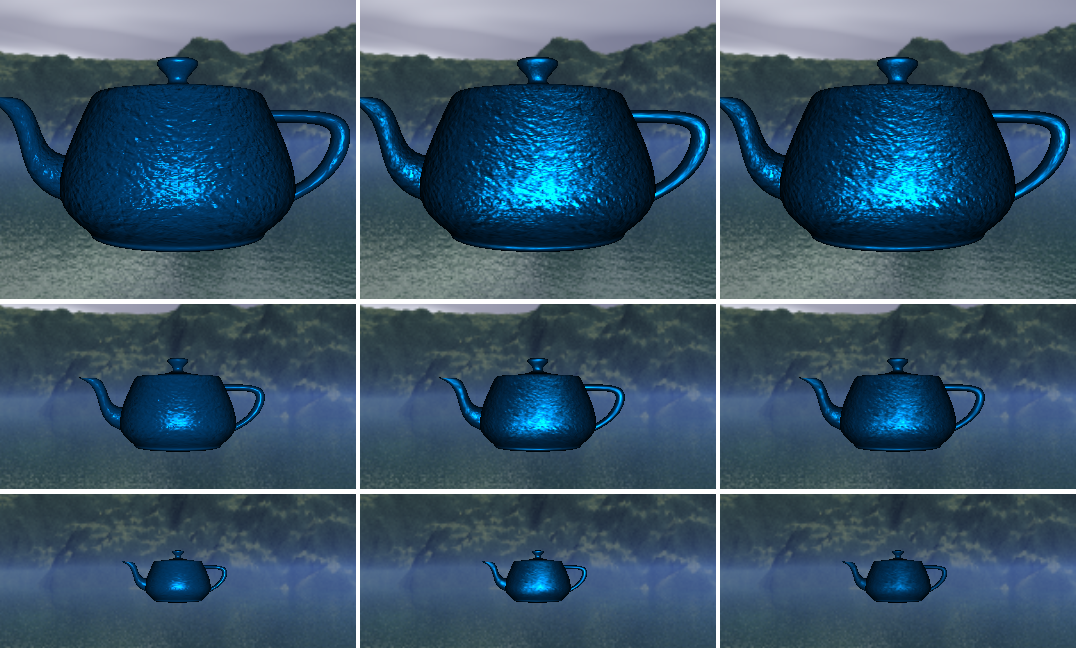
\includegraphics[width=0.49\textwidth]{figs/teapot1.png}
	\caption{Another comparison. The model used is a teapot with blue shading and light. While Bump mapping makes the teapot surface lose contrast, and LEAN preserves the highlight, the specular fading preserves the bumped surface while diminishing the highlight.}
	\label{fig:teapot1}
\end{figure}

\begin{figure}[h]
	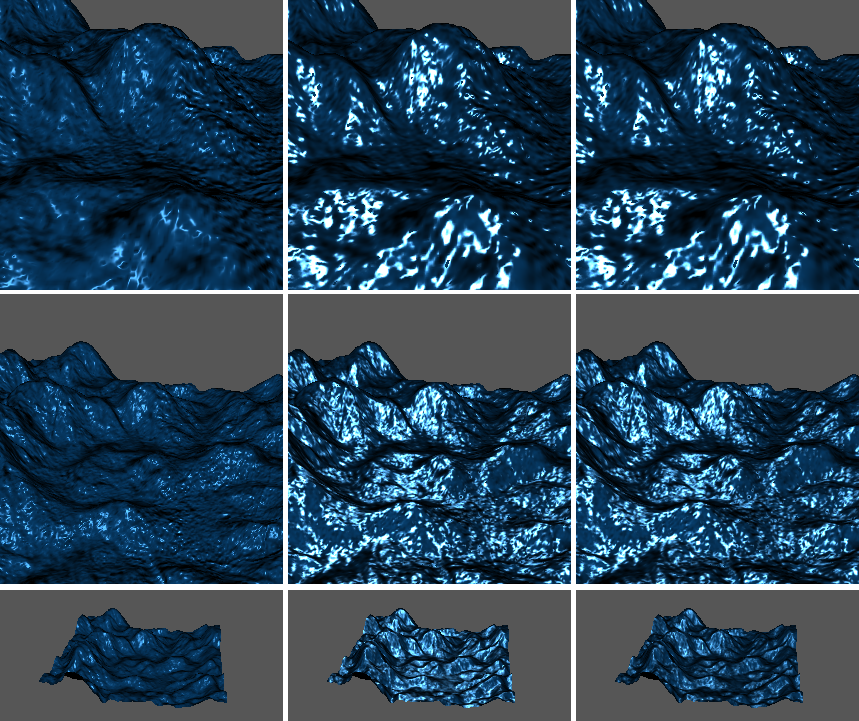
\includegraphics[width=0.49\textwidth]{figs/terrain1.png}
	\caption{Another comparison between approaches. This time with a terrain model.}
	\label{fig:terrain1}
\end{figure}

\begin{figure}[h]
	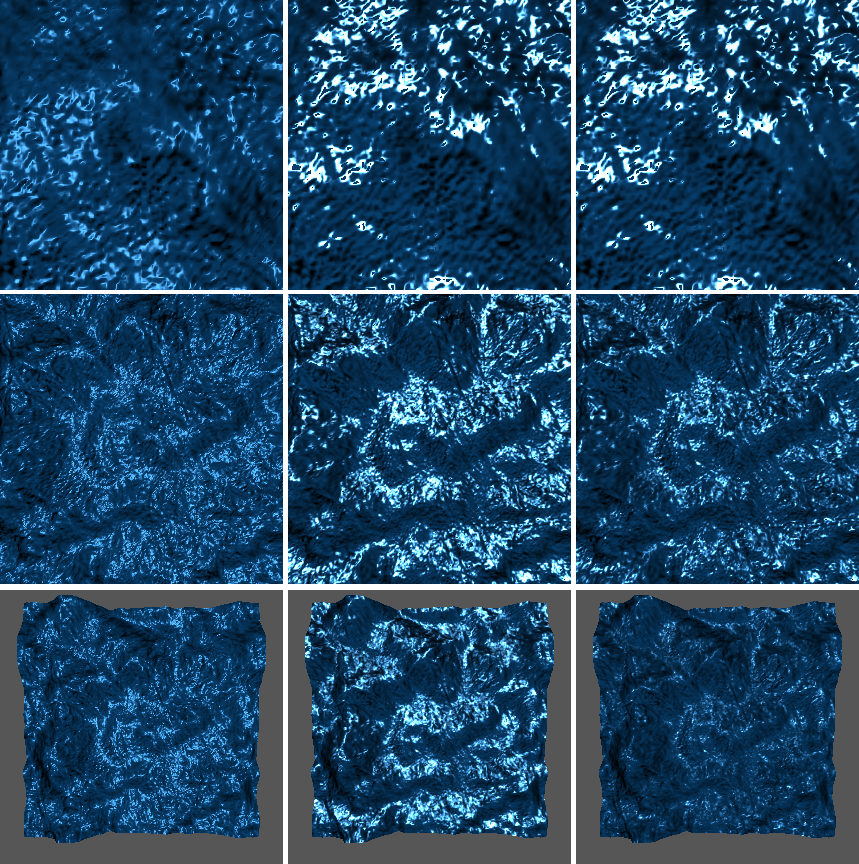
\includegraphics[width=0.49\textwidth]{figs/terrain2.png}
	\caption{The same terrain model but in a different angle.}
	\label{fig:terrain2}
\end{figure}

\begin{figure}[h]
	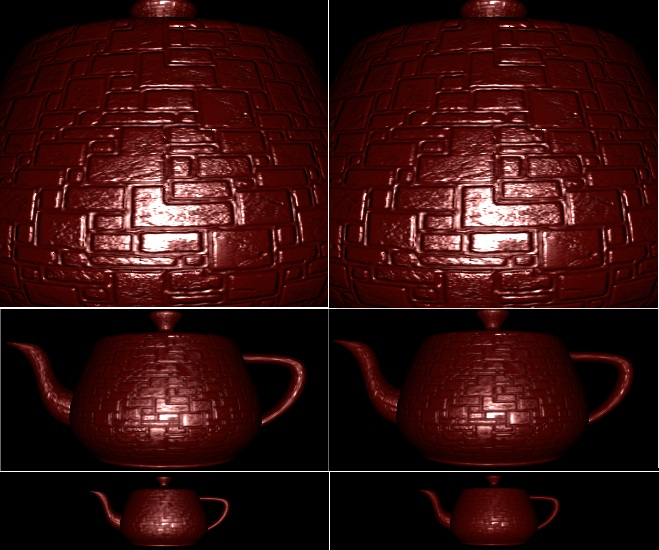
\includegraphics[width=0.49\textwidth]{figs/LS1.png}
	\caption{Comparison between LEAN and our proposed improvement using a teapot model. In the left is the traditional LEAN technique and in the right the proposed improvement. As shown in the figure, at close range they are identical, however the farther the camera is from the object, less specular highlight.}
	\label{fig:LS1}
\end{figure}

%\begin{figure}[h]
%	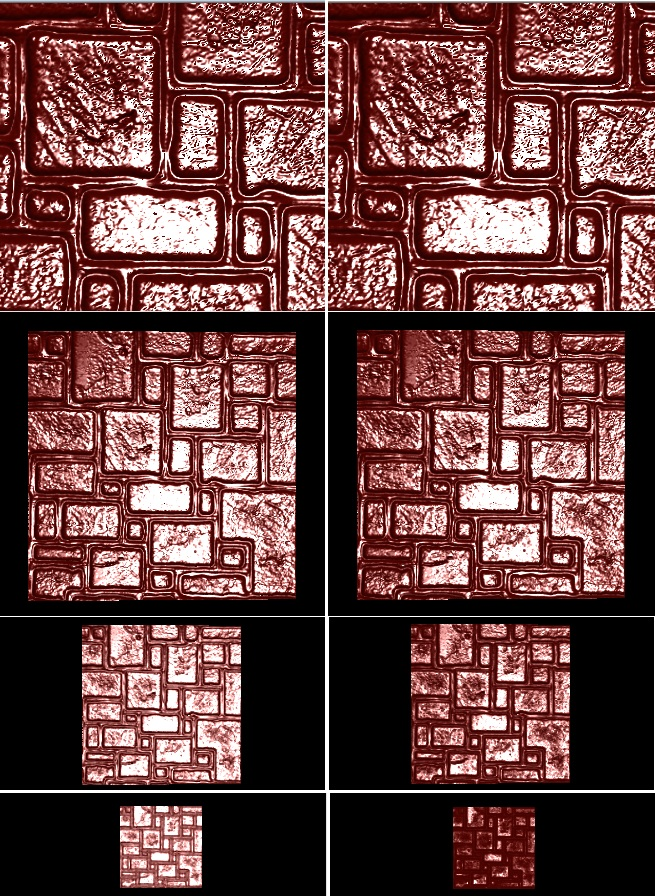
\includegraphics[width=0.49\textwidth]{figs/LS2.png}
%	\caption{Another comparison between LEAN and our proposed improvement using a square model. In the left is the t %raditional LEAN technique and in the right is LEAN with specular fading.}
%	\label{fig:LS2}
%\end{figure}


\end{document}

%==========================================
